\documentclass[12pt]{article}
\usepackage[latin1]{inputenc}
\usepackage[T1]{fontenc}
\usepackage{textcomp}
\usepackage{ae}


% \usepackage{enumerate}
\usepackage{amsmath}
\usepackage{graphicx}
\usepackage{pdfpages}

% this will produce a warning:
% LaTeX Warning: Command \@makecol has changed.
% seems to occur in combination with the setspace package.
\usepackage[stable, bottom]{footmisc}

\usepackage{color}
\definecolor{fuchsia}{rgb}{1,0,1}
\definecolor{myblue}{rgb}{0.25,0.25,0.75}
\definecolor{darkblue}{rgb}{0,0,0.75}
\usepackage[
    hyperfootnotes=false, % not compatible with footmisc pacakge
    final=true,
    colorlinks=true,
    bookmarks=true,
    bookmarksnumbered=true,
    bookmarksopen=true,
    bookmarksopenlevel=2,
    pdfstartview=FitH,
    linkcolor=myblue, citecolor=darkblue, urlcolor=myblue]{hyperref}

\title{The KrdWrd Add-on}
\author{Maria Cieschinger, Kilian Klimek, Egon Stemle}
\begin{document}
\maketitle


\section{Introduction}

"The availability of large text corpora has changed the scientific approach to language in linguistics and cognitive science" \cite{ManningSchuetze1999}.
Today, the by far richest source for authentic natural language data is the World Wide Web, and facilitating it as a data source for scientific research is imperative.

Web pages, however, can not be used for computational linguistic processing without filtering:
They contain code for processing by the Web browser, there are menus, headers, footers, form fields, teasers, out-links, spam-text -- all of which needs to be stripped.

The dimension of this task calls for an automated solution, the broadness of the problem for supervised machine learning approaches.
Part of the KrdWrd \cite{krdwrd.org} project deals with the development of appropriate methods, but they require hand-annotated pages for training.

The \textit{KrdWrd Add-on} aims at making this necessary tagging of Web pages possible.
For users, we provide accurate Web page presentation and annotation utilities in a typical browsing environment, while, for further processing, we preserve the original document and all the additional information contained therein.


\section{The Big Picture}

One of the goals of natural language processing (NLP) is to train statistical models on large amounts of data\footnote{i.e.~\textit{statistical} NLP is an integral part of NLP}. Generally speaking, the more data is available, the more accurate are the results. In the following, we will present the approach taken in the KrdWrd project, which aims at collecting and filtering large amounts of annotated linguistic data from the Web.


\subsection{Starting Point}

The World Wide Web is a virtually inexhaustible source of authentic natural language data. It therefore offers the NLP community an opportunity to train their statistical models on much larger amounts of data than was previously possible. 
Of course, the `better' the data, the more reliable are the results. 
What is meant by `better' here is that we would want our data to consist of text that allows us to find as many interesting regularities as possible, i.e.~we would want to extract text that is grammatical\footnote{Grammaticallity, of course, might not be the only valid property -- but it is certainly a well established common ground.}.

One of the main problems that we encounter when automatically extracting data from Web pages is, however, that we end up not only with full grammatical sentences or phrases, but also with a lot of other raw data. 
This includes headers, footers, advertisement, navigation information, links, etc. 
Everyone who has looked at `messy' Web pages like \url{www.web.de} will easily agree: The text that is potentially interesting for linguistic research is embedded, and almost gets lost, in a lot of text that we would most probably not want to be part of a reliable corpus for NLP, i.e. of a corpus that can be used to train statistical models. 

To sum this up, after crawling content from the Web the subsequent steps, namely, language identification, tokenising, lemmatising, part-of-speech tagging, indexing, etc. suffer from `` `large and messy' training corpora [\ldots] and interesting [\ldots] regularities may easily be lost among the countless duplicates, index and directory pages, Web spam, open or disguised advertising, and boilerplate'' \cite{Evert2008}.


\subsection{Solution/Mission}

Since it is obviously not sufficient to just extract content from Web pages, thorough preprocessing and cleaning of Web pages is crucial in order to obtain a corpus with reliable frequency data.

It is part of the KrdWrd project to develop appropriate methods for the preprocessing and cleaning of Web pages. 
These methods, however, require hand-annotated pages on which the models can then be trained. 
In the context of the seminar `Practical Natural Language Processing', we have therefore decided to develop a feasible way to tag content from Web pages as to be able to feed the result to supervised machine learning algorithms.


\section{FIASCO, CLEANEVAL and KrdWrd}

In the CLEANEVAL (CE) contest, one of the assigned tasks was very similar to the one we were pursuing in the KrdWrd project: 
Automatically clean Web pages of `noisy' data as described above. However, ``participants were largely interested in using supervised machine learning techniques [\ldots and \ldots] most systems used the HTML structure of the input page as an input to their algorithms'' \cite{BaroniChantreeKilgarriffSharoff2008} -- and so did the predecessor of the KrdWrd project, namely the FIASCO project\cite{FIASCO2007}. 
An additional requirement for our own work, then, was to improve the set-up by preserving the \textit{structural} information of Web pages, and, even more ambitiously, to \textit{annotate} the structural information of Web pages.

As a consequence, the KrdWrd project includes a Firefox Add-on that aims at making this kind of tagging of Web pages possible, i.e.~annotating the structural information of Web pages. 
We thus provide accurate page presentation and annotation utilities in a typical browsing environment for the users, \textit{while preserving} the original document and all the additional information contained therein for all different kinds of further processing, as well as for future methods that rely on the original HTML sources.


\section{What We Did}

During the semester, we accomplished the following:

\begin{itemize}
	\item Set-up a server (back-end) for different services
	\item Refined the CLEANEVAL annotation guidelines
	\item Programmed a Firefox Add-on
	\item Wrote a manual for the Add-on
	\item Made an interactive online tutorial
	\item Wrote an assignment for the class `Introduction to Computational Linguistics'
\end{itemize}


\subsection{The Server}
Experience, good practice, and practicability dictated an overall set-up where data is (initially) gathered, pre-processed, and made available from a central location. 
Furthermore, data that has been modified by users, i.e.~\textit{the} data we are interested in from users, should be available to us without much user intervention: 
Ideally, users should solely be able to \textit{work on} an assigned task without much ado about \textit{bringing it about}.  

In a nutshell, our server is a multi-purpose back-end that we use to harvest data, i.e.~grab Web pages off the web, convert them into UTF-8 encoding\cite{unicode.org}, make links on these pages relative\cite{w3.org/base}, and compile them into a corpus we can have tagged by users. 
The process starts with a list of seed terms\footnote{The seed terms were: history, coffee, salt, spices, trade road, toll, metal, silk, patrician, pirate, goods, merchant.} which are expanded by the BootCat toolkit\cite{BaroniSilvia2004} and result in a list of URLs\footnote{The term expansion resulted in 658 URLs from unique domains. i.e.~we departed from the original BootCat recipe as to only allowing one URL per domain.}. 
This list is fed to a XULRunner application\cite{xulrunner}, simply put, an automated Firefox\cite{firefox}, which retrieves the pages from the Web via our own proxy server\cite{wwwoffle}; this proxy is then used for all communication with the internet and holds, in the end, a (near\footnote{dynamically generated links are quite challenging\ldots}) copy of all pages. 

Enforcing some technical criteria on `proper' pages and manually inspecting the grabbed pages, this process resulted in a corpus of 228 pages. The server was then used to serve these pages to clients and receive tagged pages from the individual users.


\subsection{Refined Annotation Guidelines\footnotemark}\footnotetext{available from: \url{https://krdwrd.org/manual/html} -- Annotation Guidelines}

As we said earlier, in the CE contest, the removal of boilerplate was one of the assigned tasks. 
Thus, we used the CE annotation guidelines as a first approximation (cf.~\cite{cleaneval/annotation_guidelines}), and made a few substantial changes, however, because we realised that there were several cases in which the guidelines were insufficient.

One of the most important changes we made was the addition of a third tag `uncertain'. 
Originally, only the two tags `good' and `bad' were available, but it was soon apparent that on some Web pages there were passages that we did not want to be part of our corpus (i.e.~that we did not want to tag `good'), but that we did not want to throw out altogether either (i.e.~tag them as `bad'). 
We also decided to tag all captions as `uncertain'. 
One of the ideas behind this introduction of a third tag was that we might want to process these data at a later stage.

We adopted the following guidelines from the CE contest, and all of these items were supposed to be tagged `bad':

\begin{itemize}
	\item Navigation information
	\item Copyright notices and other legal information
	\item Standard header, footer, and template materials that are repeated across (a subset of) the pages of the same site
\end{itemize}

We modified the requirement to clean Web pages of internal and external link lists and of advertisement slightly: 
In our guidelines, we want \textit{all} \mbox{(hyper-)links} that are \textit{not} part of the text to be tagged as `bad'. 
This, of course, includes link lists of various kinds, but preserves links that are grammatically embedded in `good' text. 
We also restricted ourselves as to discarding advertisement from \textit{external} sites only. 
Some of the pages were pages about certain products, i.e.~advertisement, but we did not want to exclude these texts (if they fulfilled our requirements for `good' text, as defined below).

The two sorts of text that we did not exclude specifically (as the CE guidelines did), were Web-spam, such as automated postings by spammers or bloggers, and cited passages. 
Instead, we required `good' text to consist of complete and grammatical English sentences that did not contain `non-words' such as file names. 
That way, we filter out automatically generated text \textit{only if} it is not grammatical or does not make up complete sentences, and keep text that can be useful for information extraction with statistical models.

Our refined annotation guidelines still leave some small room for uncertainties (but probably \textit{all} such guidelines suffer from this problem). 
We are optimistic, however, that they are a clear improvement over the original CE guidelines and that our Web corpus will only contain complete and grammatical English sentences that contain `normal' words only.


\subsection{The KrdWrd Add-on\footnotemark}\footnotetext{available from: \url{https://krdwrd.org/trac/wiki/AddOn}}

The KrdWrd Add-on is the dual of the server back-end: 
it receives data from the server, alters the display of Web pages or supports the tagging of different parts of a page differently, and, finally, sends the annotated page back to the server for storage and further processing.

In a nutshell, the Add-on extends the functionality of the Firefox browser with a status bar menu where -- beside some administrative tasks -- the user may select to put the current browser tab into \textit{tracking mode}; 
in this mode the lovely color \textcolor{fuchsia}{fuchsia}\footnote{there is a short story behind this color: \url{https://krdwrd.org/trac/wiki/KrdWrd}}  is used to highlight the part of the page where the mouse is hovering over, and thus is subject to, tagging. 
The tagged page (or a partly tagged page, for that matter) can be (re-)submitted to the server.

\begin{center}
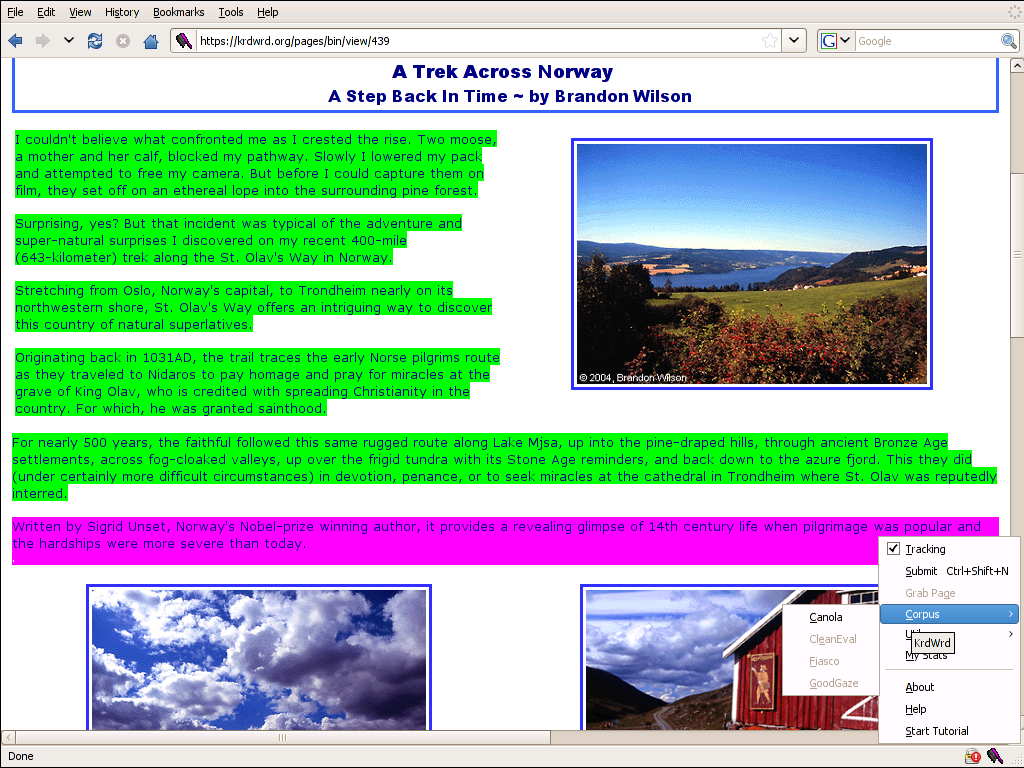
\includegraphics[width=0.85\textwidth]{images/taggingaction.png}  
\end{center}

\addtocounter{footnote}{1}
\subsection{The Manual\footnotemark[\value{footnote}]}

In the manual, we give a detailed description of all of the functionalities of the KrdWrd Add-on, and also provide tips and tricks that can help make the annotation process easier. 
It is written in such a way that someone without any kind of previous knowledge about tagging or about the Add-on can get all the necessary information, from the installation process to the submission and revision of annotated Web pages (at least, that is the idea).

The manual has the following structure and can be viewed in a browser or can be downloaded as a pdf file\footnotemark[\value{footnote}]:
\footnotetext{available from: \url{https://krdwrd.org/trac/wiki/AddonManual}}


\begin{itemize}
	\item Introduction
	\item Getting Started
		\begin{itemize}
			\item First Steps
			\item The Statusbar Menu
		\end{itemize}
	\item How to Tag Pages
		\begin{itemize}
			\item Annotation Guidelines
			\item Examples - Easy
			\item Examples - Medium
			\item Examples - Hard
		\end{itemize}
	\item Tips \& Tricks
		\begin{itemize}
			\item Keyboard Shortcuts
			\item How and When to Use Propagate
			\item How to \textit{Undo}
		\end{itemize}
	
\end{itemize}

We included selected samples of authentic pages in the Section `How to Tag Pages' and ranked them according to their difficulty to be tagged correctly. 
For further practice, we also developed an interactive tutorial that can be viewed online.


\subsection{The Interactive Online Tutorial}

The interactive tutorial can be accessed from the status bar by clicking `Start Tutorial', and is designed to practice the annotation process itself and to learn how to use the three different tags correctly. 
Eleven sample pages are displayed one after another, ranging from easy to difficult (these are the same samples as in the 'How to Tag Pages' Section of the manual).

The user is asked to tag the displayed pages according to the guidelines presented in the manual. 
We inserted a validation step between the clicking of `Submit' and the presentation of the next page, giving the user feedback on whether or not s/he used the tags correctly. 
Passages that are tagged corresponding to our own annotations are then displayed in a light-coloured version of the original tag, i.e.~text correctly tagged as `bad' will be light-red, `good' text will be light-green, and text that was tagged correctly as `uncertain' will be light-yellow.
The passages whose annotation \textit{differs} from our own are displayed in the colour in which they should have been tagged, using the normal colours, i.e.~red, green, and yellow. After clicking `Next Page' on the right top of the screen, the next page will be shown.

If a user should decide to quit the interactive tutorial before having tagged all eleven sample pages, the next time s/he opens the tutorial, it will begin with the first of the pages that have not been tagged, yet. 
And should a user want to start the tutorial from the beginning, s/he can delete previous annotations via `My Stats' in the status bar. 
Then, the next time the tutorial is opened, it will start from the very beginning. 
By pressing `Start Tutorial' in the status bar during the practice and \textit{before} the submission of the current page, that same page will be displayed again, un-annotated. 
When using `Start Tutorial' \textit{after} a page's submission and before clicking `Next Page' in the notification box at the top, the next page of the tutorial will be shown.

As stated above, it is our goal that the interactive tutorial will help users getting used to the annotation process, and we are also optimistic that it helps understanding and correctly applying the tagging guidelines as presented in the manual.


\subsection{The Assignment}

Finally, our efforts were incorporated into an assignment for the class `Introduction to Computational Linguistics' where -- from a maximum number of 100 students -- 68 completed a substantial part of the assignment, i.e.~their effort was worth at least 50\% of the assignment's total regular credits\footnote{Actually, the worst accomplishment was still worth 70\%.} .
The assignment was handed out July 7th, was due July 18th, and consisted of two exercises:
\begin{enumerate}
	\item The first task was to complete the interactive online tutorial, i.e.~the students had to go through the eleven sample pages, annotate them, and -- ideally -- think about the feedback. This task was worth 20\% of the credits.
	\item The second task was to tag pages from our assembled corpus; 15 tagged pages were worth 80\% of the credits and 10 additional pages were worth an extra that was counted towards the credits of all other homework assignments, i.e.~students could make up for `lost' credits\footnote{As a matter of fact, 43 students received the total of 100\% regular credits + 100\% extra credits.}.
\end{enumerate}

%\subsection{Technical Aspects?}

%(from the slides:)

%\begin{itemize}
%	\item A shared Debian/GNU Linux Server with a shared Apache Web server \cite{debian.org}
%	\item A dedicated Trac, i.e. an enhanced wiki and issue tracking system for software development projects \cite{trac}
%	\item A dedicated svn, i.e. an open-source revision control system for all documentation and all programme code \cite{subversion}
%	\item A WWWOffle proxy server to keep a (quite) pure version of the pages to be tagged \cite{wwwoffle}
%	\item An XULRunner application to harvest the pages \textit{through} the proxy -- as if they were viewed by a user \cite{xulrunner}
%	\item JavaScript\cite{javascript}, Python\cite{python}, Perl\cite{perl}, Bash-scripting\cite{bash} for the necessary front- and back-ends
%	\item An SQLile3\cite{sqlite} self-contained, embeddable, zero-configuration SQL database engine for the (less) pure version of the pages to be tagged and the users' annotations
%	\item \ldots
%\end{itemize}

\subsection{Task Division}

Egon Stemle worked primarily on the technical aspects, wrote the assignment, and organized everything. Maria Cieschinger and Kilian Klimek were mainly responsible for writing the manual and for selecting Web pages that could be used in the interactive tutorial.

%\section{References}
\addcontentsline{toc}{section}{References}
\nocite{*}

\footnotesize
\bibliographystyle{myalphaurl}
\bibliography{2008.pNLP}
\normalsize

\newpage
\pagestyle{empty}
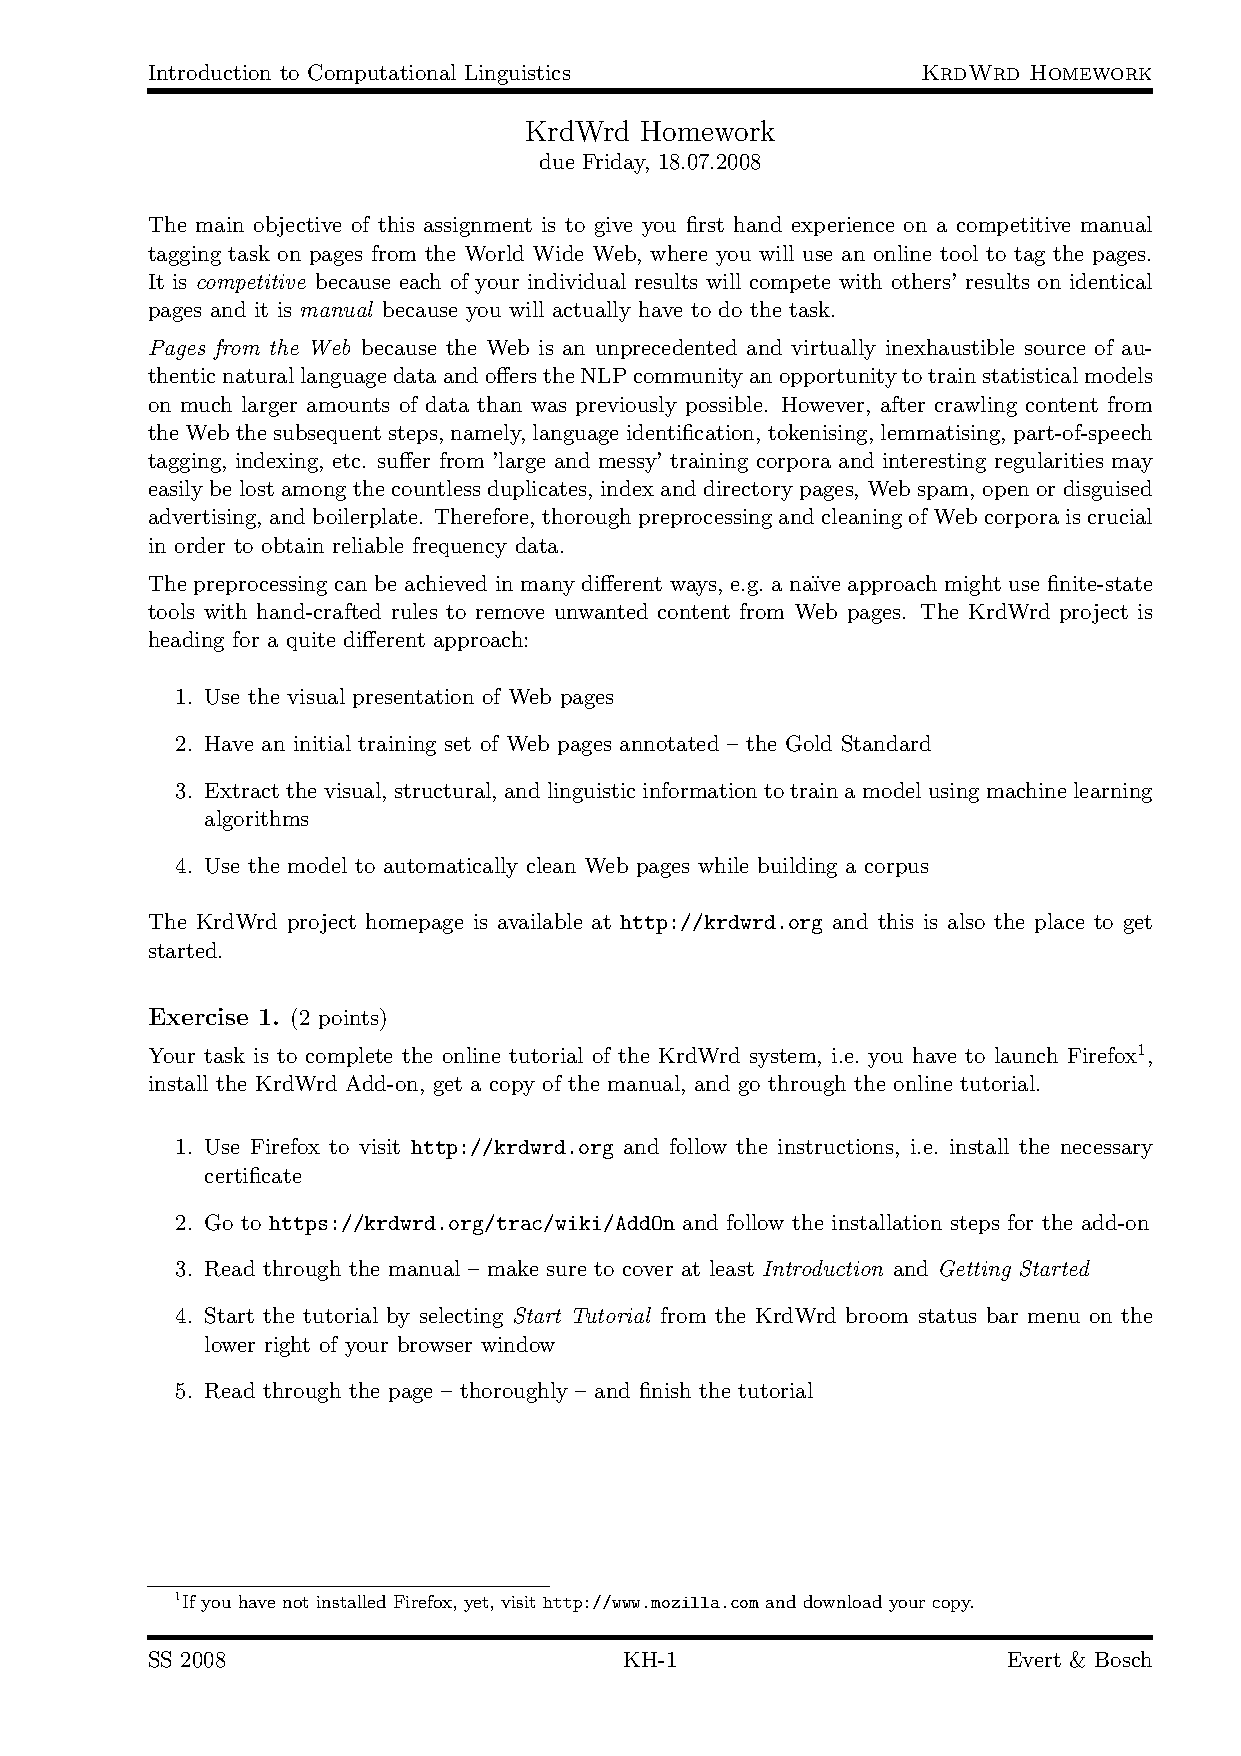
\includepdf[pages=-, frame, scale=0.9]{images/homework_krdwrd.pdf}
\addcontentsline{toc}{section}{Appendix}
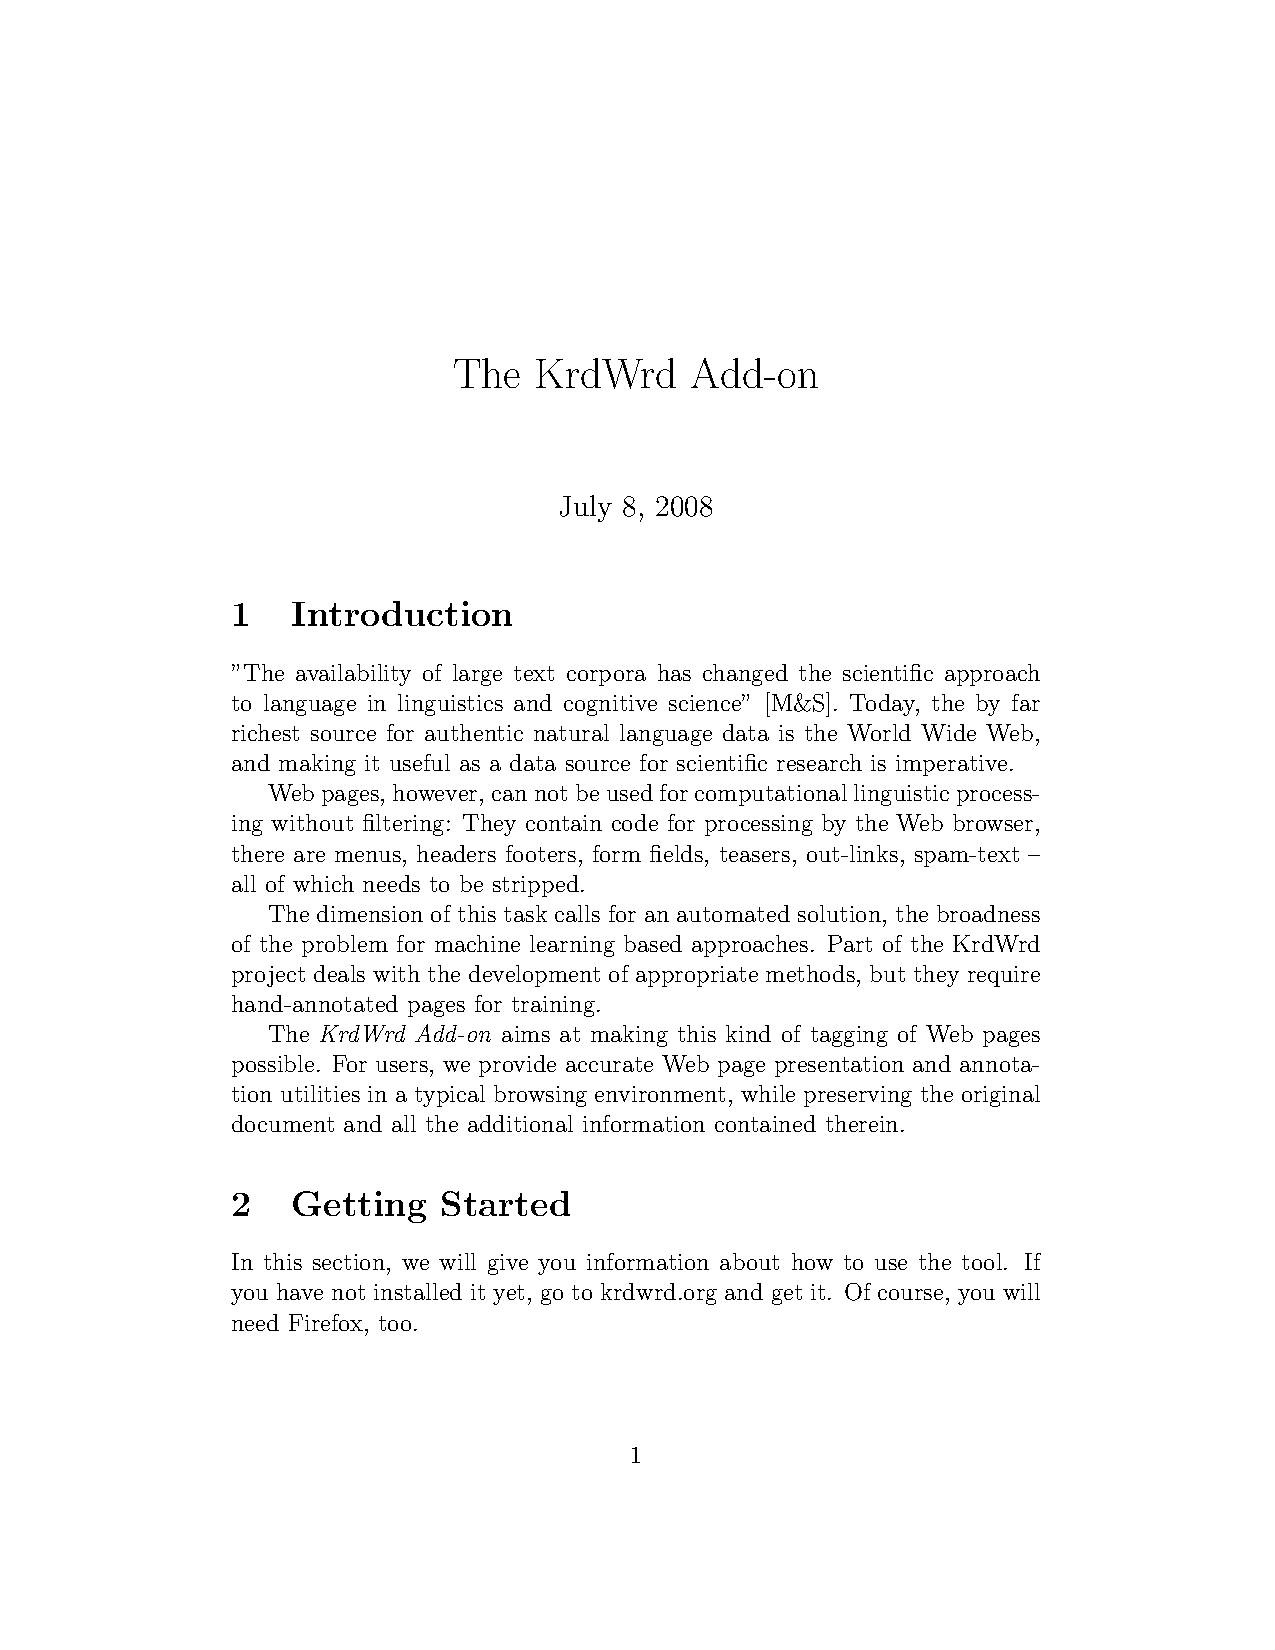
\includepdf[pages=-, frame, scale=0.9]{images/manual.pdf}

\end{document}
